\setchapterpreamble[ur]{
  \dictum
  [Michèle Audin, \textit{Conseils aux auteurs de textes mathématiques}]
  {Un texte mathématique est, d’abord, un texte.}
  \vspace{1em}
}



\chapter{Writing text}

% According to \cite{mathoverflow_text} and Google~Translate the above quote may be translated as follows:
% \begin{center}
%   \enquote{A mathematical text is, before everything else, a text.}
% \end{center}
In this chapter we will talk about the more text focused aspects of writing a mathematical text with {\LaTeX}.
We will in particular talk about the interplay between mathematical content and the text that surrounds it.




\section{Obey orthography}
\label{a mathematical text is a text}

A mathematical text has to obey the rules of the language that is it written in (e.g.~English, French, German or Russian).
It also means that a mathematical formula is part of the surrounding text, and has to be treated as such.





\section{A sentence ends with punctuation}

\Cref{a mathematical text is a text} has an important consequence:
If a sentence ends with a formula, then this formula need to be followed by some kind of punctuation (in most cases by a full point).
The following example does it very wrong:
\begin{showlatex}*{Very wrong punctuation in an equation}
It follows that
\[
  a^2 + b^2 = c^2
\]
.
This formula is important.
\end{showlatex}
The next example is also wrong:
\begin{showlatex}*{Wrong punctuation in an equation~I}
It follows that
\[
  a^2 + b^2 = c^2
\]
This formula is important.
\end{showlatex}
The following is still wrong:
\begin{showlatex}*{Wrong punctuation in an equation~II}
It follows that:
\[
  a^2 + b^2 = c^2
\]
This formula is important.
\end{showlatex}
The following example finally does it right:
\begin{showlatex}*{Right punctuation in an equation}
It follows that
\[
  a^2 + b^2 = c^2.
\]
This formula is important.
\end{showlatex}
But it is even better if we add some slight spacing between the formula and the period.
\begin{showlatex}*{Best punctuation in an equation}
It follows that
\[
  a^2 + b^2 = c^2 \,.
\]
This formula is important.
\end{showlatex}
This last approach is taken from \cite{tex_period}, which we strongly encourage the reader to check out.






\section{Punctuation in commutative diagrams?}

There is some disagreement in the mathematical community about whether a commutative diagram is allowed to include punctuation coming from the surrounding text.
The author is of the opinion that a commutative diagram should not contain any such punctuation.
So when including a commutative diagram one has to either finish up the preceeding sentence beforehand, or has to incorporate the diagram in such a way that it contains no punctuation of the surround text.
\begin{showlatex}{Finishing the sentence before the commutative diagram}
  We consider the following commutative diagram:
  \[
    \begin{tikzcd}
        A
        \arrow{r}
        \arrow{d}
      &
        A'
        \arrow{d}
      \\
        C
        \arrow{r}
      &
        C'  
    \end{tikzcd}
  \]
  The horizontal arrows in this diagram are isomorphisms.
\end{showlatex}
\begin{showlatex}{Incorporating the commutative diagram in the sentence}
  In the commutative diagram
    \[
    \begin{tikzcd}
        A
        \arrow{r}
        \arrow{d}
      &
        A'
        \arrow{d}
      \\
        C
        \arrow{r}
      &
        C'  
    \end{tikzcd}
  \]
  both horizontal arrows are isomorphisms.
\end{showlatex}





\section{Know your hypen and dashes}

In {\LaTeX} there are (at least) four kind of line-like symbols which need to be distinguished, see \cref{dash list}.
\begin{table}[tb]
  \begin{center}
  \begin{tabular}{lll}
    \toprule
    \textbf{name}
    &
    \textbf{code}
    &
    \textbf{output}
    \\
    \midrule
    hypen
    &
    \inlinecode{-}
    &
    -
    \\
    endash
    &
    \inlinecode{--}
    &
    --
    \\
    emdash
    &
    \inlinecode{---}
    &
    ---
    \\
    minus sign
    &
    \inlinecode{\$-\$}
    &
    $-$
    \\
    \bottomrule
  \end{tabular}
  \end{center}
  \caption{Kinds of hypen and dashes.}
  \label{dash list}
\end{table}
Each of these line-like symbols plays its own role, but these roles depend both on language and on convention.
For mathematical writing in English the following usages are important:
\begin{itemize}
  \item
    For \enquote{$n$-dimensional} and \enquote{$3$-manifold}, use the hypen.
  \item
    For combining names as in \enquote{Cauchy--Schwarz inequality} use the endash.
  \item
    To interupt a sentence---as done here---use either the emdash without surround space.
    If you’re British -- or like to pretend that you are -- use the endash surrounded by space.
\end{itemize}
For more information about the use of hypen and dashes in the English language we refer to \cite[6.75--6.94]{chicago}.

To underline how language dependent the usuage of hypen and dashes we consider in \cref{cgc names} how the the Clebsch--Gordan are called in different languages, as taken from Wikipedia.
(We use the font~\texttt{Noto Serif CJK JP} for all examples to allow a better comparison.)
\begin{table}[tb]
  \begin{center}
  \begin{tabular}{@{}lll@{}}
    \toprule
    \textbf{language}
    &
    \textbf{name}
    &
    \textbf{dash used}
    \\
    \midrule
    English
    &
    \multilang{Clebsch–Gordan coefficients}
    &
    endash
    \\
    German
    &
    \multilang{Clebsch-Gordan-Koeffizienten}
    &
    hyphen
    \\                                                      
    French
    &
    \multilang{coefficients de Clebsch-Gordan}
    &
    hyphen
    \\
    Dutch
    &
    \multilang{Clebsch-Gordan-coëfficienten}
    &
    hyphen
    \\
    Russian
    &
    \multilang{Коэффициенты Клебша — Гордана}
    &
    emdash
    \\
    Japanese
    &
    \multilang{クレブシュ–ゴルダン係数}
    &
    endash
    \\
    \bottomrule
  \end{tabular}
  \end{center}
  \caption{Clebsch--Gordan coefficients in different languages.}
  \label{cgc names}
\end{table}





\section{Use non-breakable space}
\label{non-breakable space}

If two expressions in text mode are separated by a space or a hypen then {\LaTeX} may separate the resulting output by a line break.
But in many situations such line breaks are unwanted, or downright wrong.
\begin{itemize}
  \item
    In abbreviations like~\enquote{Prof.~Doe}.
  \item
    In combinations of words and numbers like~\enquote{Lemma~5}.
  \item
    In combinations of mathematics and words like~\enquote{$3$\nobreakdash-dimensional}.
\end{itemize}
In such cases one can tell {\LaTeX} that no line break must occur:
\begin{itemize}
  \item
    If the tilde symbol~\inlinecode{\customtexttilde}, also know as a \emph{tie}, is used instead of a simple whitespace, then no line break will occur.
    Consider the following example:
    \begin{showlatex}*{An unwanted line break at a space}
It follows from the above Lemma 5 that the integer $2$ is prime.
    \end{showlatex}
    We don’t want a line break to occur in~\enquote{Lemma~5} and thus use an unbreakable space.
    One should also make sure that no line break occurs in the expression~\enquote{integer~$2$}
    \begin{showlatex}*{Using~\inlinecode{\customtexttilde} to prevent unwanted line breaks at spaces}
It follows from the above Lemma~5 that the integer~$2$ is prime.
    \end{showlatex}
  \item
    If a hypen should not be broken then~\commandname{nobreakdash} can be used.
    Consider the following example:
    \begin{showlatex}{An unwanted line break at a hypen}
The sphere $S^2$ will be our very first non-trivial example of a smooth $2$-manifold (without boundary).
    \end{showlatex}
    To prevent a line break at the hypen we put~\commandname{nobreakdash} before it:
    \begin{showlatex}{Using~\commandname{nobreakdash} to prevent unwanted line breaks at hypens}
The sphere $S^2$ will be our very first non-trivial example of a smooth $2$\nobreakdash-manifold (without boundary).
    \end{showlatex}
    Note that 
    The command~\commandname{nobreakdash} also works with other kinds of dashes, like~\inlinecode{--} and~\inlinecode{---}.
%   TODO: Add an example
\end{itemize}





\section{Use proper spacing after dots}
\label{spacing after dots}



\subsection{The basic problem}

Not all periods are treated equally by {\LaTeX}:
If a period is both followed by whitespace and not preceded by an uppercase letter then {\LaTeX} will assume that this period is supposed to end a sentence.
It will some introduce some additional space following this period.
The effect of this can be seen in \cref{period spacing}.
(The two segments are always separated by a single space, and we have scaled the text by a factor of~$3.5$ for readability.)
\begin{table}
  \begin{center}
  \begin{tabular}{@{}r@{\hskip 2.7em}r@{\hskip 2.7em}l@{\hskip 2.7em}l@{}}
    \toprule
    \multicolumn{2}{c}{\textbf{right aligned}}
    &
    \multicolumn{2}{c}{\textbf{left aligned}}
    \\
    \cmidrule(r{2.7em}){1-2}\cmidrule{3-4}
    \scalebox{3.5}[3.5]{x. x}
    &
    \scalebox{3.5}[3.5]{x. X}
    &
    \scalebox{3.5}[3.5]{x. x}
    &
    \scalebox{3.5}[3.5]{X. x}
    \\
    \scalebox{3.5}[3.5]{X. x}
    &
    \scalebox{3.5}[3.5]{X. X}
    &
    \scalebox{3.5}[3.5]{x. X}
    &
    \scalebox{3.5}[3.5]{X. X}
    \\
    \bottomrule
  \end{tabular}
  \end{center}
  \caption{Spacings after a period.}
  \label{period spacing}
\end{table}

We can see from the first two columns of~\cref{period spacing} (by considering the positions of the periods) that the spacing in~\enquote{\inlinecode{x. *}} is larger then the corresponding spacing in~\enquote{\inlinecode{X. *}}.
This happens because {\LaTeX} thinks that the period in~\enquote{\inlinecode{x. *}} is supposed to end a sentence.
We can also see from the first two tables that this difference of spacing occurs both if the following letter is lower case and if it is upper case.
We can see from the third and fourth column that the amount of additional spacing does not depenend on whether the following letter is in lower case or upper case.



\subsection{Solution}

We can use the command~\enquote{\commandname{ }} to tell~{\LaTeX} that a preceeding period is not meant to end a sentence, and we can similarly use~\enquote{\commandname{{\tbs}@}} to tell {\LaTeX} that the following period is shall end the sentence.
Consider the following example:
\begin{showlatex}{Proper spacing after periods}
Imagine now some old and long-dead English kings, e.g.\ Henry III and Henry IV\@.
(Kings not named Henry are also okay.)
\end{showlatex}
Note that in the above example one should also use ties~\inlinecode{\customtexttilde} (as explained in \cref{non-breakable space}) to ensure that the Henries don’t get separated from their number:
\begin{showlatex}{Proper spacing after periods, and using~\inlinecode{\customtexttilde}}
Imagine now some old and long-dead English kings, e.g.\ Henry~III and Henry~IV\@.
(Kings not named Henry are also okay.)
\end{showlatex}

It should be pointed out that if a problematic period is followed by a closing parenthesis, a closing brecket or quotations marks then then the problematic spacing will still occur after these symbols.
Lets consider the following example (where we use the forbidden \commandname{\tbs} to compare the versions).
\begin{showlatex}{Spacings after periods followed by parentheses or quotation marks}
Many colours (e.g. red, blue, etc.) are supported by \enquote{ColorX}. Even purple! \\
Many colours (e.g.\ red, blue, etc.) are supported by \enquote{ColorX}. Even purple! \\
Many colours (e.g.\ red, blue, etc.)\ are supported by \enquote{ColorX}. Even purple! \\
Many colours (e.g.\ red, blue, etc.)\ are supported by \enquote{ColorX}\@. Even purple!
\end{showlatex}

The problem of a sentence ending with an upper case letter does not occur if this letter is in math mode.
\begin{showlatex}{Upper case mathematics followed by a period}
Let $f$ be an endomorphism of $X$.
Then $f$ is an isomorphism or $f = 0$.\\
Let $f$ be an endomorphism of $X$\@.
Then $f$ is an isomorphism or $f = 0$.\\
Let $f$ be an endomorphism of $X$.\ 
Then $f$ is an isomorphism or $f = 0$.
\\
Let $f$ be an endomorphism of $\operatorname{X}$.
Then $f$ is an isomorphism or $f = 0$.\\
Let $f$ be an endomorphism of $\operatorname{X}$\@.
Then $f$ is an isomorphism or $f = 0$.\\
Let $f$ be an endomorphism of $\operatorname{X}$.\ 
Then $f$ is an isomorphism or $f = 0$.
\end{showlatex}

In view of \cref{non-breakable space} we get a problem:
What if we want the space after an abbreviation, as in~\enquote{i.e.~word}, not to be broken?
Should we then write~\inlinecode{i.e.{\tbs} word} or~\inlinecode{i.e.{\customtexttilde}word}?

In this case we write~\inlinecode{i.e.{\customtexttilde}word}, since the tie~\inlinecode{\customtexttilde} already contains the effect of~\enquote{\inlinecode{{\tbs} }}.
Consider for this the following example:
\begin{showlatex}{Spacing of~\inlinecode{\customtexttilde} and~\enquote{\inlinecode{{\tbs} }}}
Let $M$ be a $2$-manifold, e.g. $M = S^2$-dimensional. \\
Let $M$ be a $2$-manifold, e.g.\ $M = S^2$-dimensional. \\
Let $M$ be a $2$-manifold, e.g.~$M = S^2$-dimensional.
\end{showlatex}

To summarize this \lcnamecref{spacing after dots}:
As long as words are written, no problem occur.
If an abbreviation or some non-word things appear one should pay heed to periods which may occur.
The most of these special cases are covered by paying attention to~\enquote{i.e.~words} and~\enquote{e.g.~words}.

We refer to \cite[19.5.1, 19.6]{latex2e_manual} for more information on this topic.





\section{Lists contain punctuation}

Text that is organized using list environments still obeys the rules of punctuation.
Consider the following counterexample:
\begin{showlatex}{Wrong punctuation in lists}
  A set $B$ is a basise of $V$ if
  \begin{enumerate}
    \item
      $B$ is linearly independent
    \item
      $B$ is a generating set
  \end{enumerate}
\end{showlatex}
To figure out the correct punctuation simply remove the surrounding list and consider the resulting text.
In the above example this gives the following:
\begin{center}
  A set $B$ is a basis of $V$ if $B$ is linearly independent $B$ is a generating set
\end{center}
This is not a proper sentence, and should be the following instead:
\begin{center}
  A set $B$ is a basis of $V$ if $B$ is linearly independent and $B$ is a generating set.
\end{center}
The above counterexample should hence read as follows:
\begin{showlatex}{Right punctuation in lists~I}
  A set $B$ is a basise of $V$ if
  \begin{enumerate}
    \item
      $B$ is linearly independent and
    \item
      $B$ is a generating set.
  \end{enumerate}
\end{showlatex}
There are also some other acceptable versions:
\begin{showlatex}{Right punctuation in lists~II}
  A set $B$ is a basise of $V$ if it satisfies the following conditions:
  \begin{enumerate}
    \item
      $B$ is linearly independent.
    \item
      $B$ is a generating set.
  \end{enumerate}
\end{showlatex}





\section{Don’t use \texttt{\tbs\tbs} or \texttt{{\tbs}newline}}

The proper way to separate two succeeding paragraphs in {\LaTeX} is to leave an empty line between them.
\begin{showlatex}*{New pagragraphs done right}
This is the first pagraph.
It consists of multiples lines to make this example better.

This is a second paraph.
It also consists of multiple lines to make this example even more better.

This one is the third and last paragraph in this example.
It also consists of multiple lines.
\end{showlatex}
Note that a new paragraph starts indented.

The use of~\commandname{\tbs} or~\commandname{newline} doesn’t actually end a paragraph but instead forces {\LaTeX} to continue at the beginning of a new line.
\begin{showlatex}*{New \enquote{pagragraphs} done wrong}
This is the first paragraph in a counterexample.\\
This is not a new paragraph.
The text was just forced to start a new line.\newline
This one is also not a new paragraph.
But this whole thing looks ugly.
\end{showlatex}
The use of \texttt{\tbs\tbs} and \texttt{{\tbs}newline} is only for starting new rows in matrices, tables and arrays.
Don’t use is to separate paragraphs.





\section{Don’t break inline math}
\label{breaking inline math}

When inline formulas or equations are too long or badly placed then it can happen that a line break occurs, tearing the formula apart:
% standard values for penalities, for the demonstration
\begin{showlatex}[before lower = {\binoppenalty=100}, after lower = {\binoppenalty = \maxdimen}]{Line break in inline math}
The most important formula of all times is without a doubt is my mind $1 + 2 + 3 + 4 = 10 - 5$.
Truly a work of genius!
\end{showlatex}
This horrible affront to nature can thankfully be completely stopped by raising the corresponding penalties to their (literal) maximum:
\begin{showlatex}{Preventing inline math in inline math}
% in the preamble:
\binoppenalty = \maxdimen
\relpenalty = \maxdimen
% in the main text:
The most important formula of all times is without a doubt is my mind $1 + 2 + 3 + 4 = 10 - 5$.
Truly a work of genius!
\end{showlatex}
(One can also lower these penalities to ensure a really bad looking first example.)





\section{Don’t begin a sentence with a mathematics}

Don’t begin a sentence with a mathematical symbol.
Consider the following example:
\begin{showlatex}{Mathematics at the beginning of a sentence}
\begin{theorem}
  $\mathbf{Mod}(R)$ is an abelian category.
\end{theorem}
\end{showlatex}
Instead do the following:
\begin{showlatex}{No mathematics at the beginning of a sentence}
\begin{theorem}
  The category $\mathbf{Mod}(R)$ is abelian.
\end{theorem}
\end{showlatex}

An exception to the above rule are lists, in which short entries may start with a math symbol.
Consider for this the following example.
\begin{showlatex}{List items beginning with mathematics}
Let $V$ be a finite dimensional vector space.
Let $U$ and $W$ be two linear subspaces of $V$ of complementary dimensions, i.e.\ such that $\dim V = \dim U + \dim W$.
Then the following conditions are equivalent:
\begin{enumerate}[label = \roman*)]
  \item
    $V = U \oplus W$,
  \item
    $V = U + W$,
  \item
    $V = U \cap W$.
\end{enumerate}
\end{showlatex}





\section{Don’t put two formulas next to each other}

One should not put two mathematical formulas right next to each other.
Consider the folloing example:
\begin{showlatex}{Not properly separating mathematics}
Then $f^2 = g$,$f$ is differentiable and $f = \exp(h)$.
\end{showlatex}
Thu human eye (and brain) parses this sentence as follows:
\begin{center}
  Then
  \quad
  $f^2 = g$,$f$
  \quad
  is differentiable and
  \quad
  $f = \exp(h)$.
\end{center}
But this betrays the actual content of the sentence.
This problem can be fixed by introducing some text.
One solution is the following:
\begin{showlatex}{Properly separating mathematics~I}
Then $f^2 = g$, the function $f$ is differentiable and $f = \exp(h)$.
\end{showlatex}
This sentence is parsed as follows:
\begin{center}
  Then
  \quad
  $f^2 = g$,
  \quad
  the function
  \quad
  $f$
  \quad
  is differentiable and
  \quad
  $f = \exp(h)$.
\end{center}
The following is another solution:
\begin{showlatex}{Properly separating mathematics~II}
The function $f$ satisfies $f^2 = g$, it is differentiable and $f = \exp(h)$.
\end{showlatex}
This sentence is parsed as follows:
\begin{center}
  The function
  \quad
  $f$
  \quad
  satisfies
  \quad
  $f^2 = g$,
  \quad
  it is differentiable and
  \quad
  $f = \exp(h)$.
\end{center}







\section{Use \commandtt{text}}

When text needs to be used in math mode use \commandtt{text}.
The following is horrible:
\begin{showlatex}{Missing text in math mode}
Let $A \coloneqq \{ x \in [0,1] : x \; is \; rational \}$.
\end{showlatex}
This next one looks a bit better, but is still not okay:
\begin{showlatex}[label = {wrong math mode position}]{Wrong way of using text in math mode}
Let $A \coloneqq \{ x \in [0,1] : x \text{ is rational} \}$.
\end{showlatex}
Instead do this:
\begin{showlatex}[label = {right math mode position}]{Right way of using text in math mode}
Let $A \coloneqq \{ x \in [0,1] : \text{$x$ is rational} \}$.
\end{showlatex}
Note that the right code reflects the structure of the displayed expression:
Indeed, the diagram in \cref{structure tree of definition} shows the structure of the given expression.
\begin{figure}[tb]
  \begin{center}
    % the following diagram uses the "trees" library
    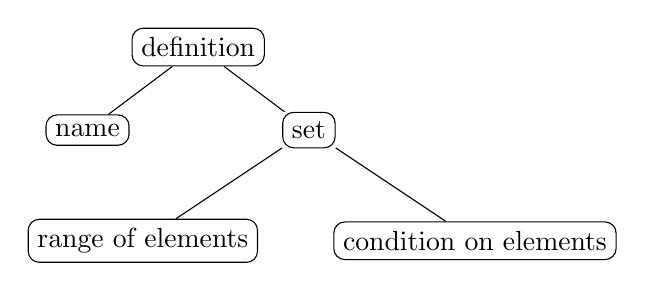
\begin{tikzpicture}[
      every node/.style = {shape=rectangle, rounded corners, draw, align=center, level distance = 5em},
      level 1/.style = {sibling distance = 8em, level distance = 3em},
      level 2/.style = {sibling distance = 12em, level distance = 4em}
      ]
      \node {definition}
        child { node {name} }
        child { node {set} 
                child { node {range of elements} }
                child { node {condition on elements} }
              }
        ;
    \end{tikzpicture}
  \end{center}
  \caption{Structure tree of the definition.}
  \label{structure tree of definition}
\end{figure}
To get the right kind of code we assign to each node of this diagram the desired content, and whether this node is mathematics or text.
If a node contains both mathematics and text then it is primary a text, which just happens to contain some mathematics.
We arrive at the diagram in \cref{structure tree of math}.
\begin{figure}[tb]
  \begin{center}
    % the following diagram uses the "trees" library
    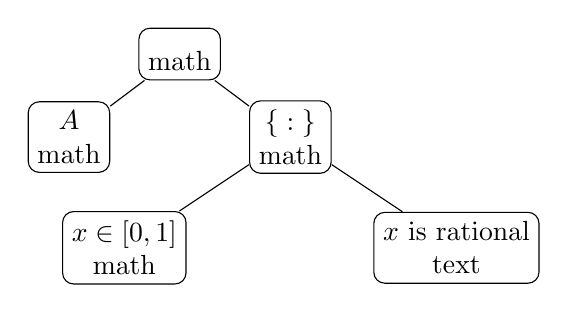
\begin{tikzpicture}[
      every node/.style = {shape=rectangle, rounded corners, draw, align=center, level distance = 5em},
      level 1/.style = {sibling distance = 8em, level distance = 3em},
      level 2/.style = {sibling distance = 12em, level distance = 4em}
      ]
      \node {$\coloneqq$ \\ math}
        child { node {$A$ \\ math} }
        child { node {$\{ \; : \; \}$ \\ math} 
                child { node {$x \in [0,1]$ \\ math} }
                child { node {$x$ is rational \\ text} }
              }
        ;
    \end{tikzpicture}
  \end{center}
  \caption{Structure tree of the matematical expression.}
  \label{structure tree of math}
\end{figure}
By transforming this diagram node-wise into code we arrive at \cref{right math mode position}.
Note that both the nodes~\enquote{$x \in [0,1]$} and~\enquote{$x$ is rational} both contain mathematics, but that the second is actually a text.
It is therefore not proper to combine these two math modes, as done in \cref{wrong math mode position}.





\section{Put space between math and text}

Sometimes a single line of displayed mathematics end with some text, as in the following example.
\begin{showlatex}{Wrong spacing around text in math mode~I}
Therefore
\[
  g h g^{-1}
  =
  h
  \text{for all $g, h \in G$}.
\]
\end{showlatex}
In such a case one needs to put space between the mathematics and the text.
This space should not be part of the text:
\begin{showlatex}{Wrong spacing around text in math mode~II}
Therefore
\[
  g h g^{-1}
  =
  h
  \text{ for all $g, h \in G$.}
\]
\end{showlatex}
Instead it should be put between the formula and the text.
In the above example, where a single block of mathematics is follows by a single block of text which contains quantifiers for the previous formula, one should put a \commandname{qquad}:
\begin{showlatex}{Right spacing arond text in math mode~I}
Therefore
\[
  g h g^{-1}
  =
  h
  \qquad
  \text{for all $g, h \in G$.}
\]
\end{showlatex}
Sometimes two blocks of mathematics are separated by a short text.
In this case one should use~\commandname{quad} on both sides of the text:
\begin{showlatex}{Right spacing around textt in math mode~II}
That $gh = hg$ can equivalently be expressed as
\[
  g h g^{-1} = h
  \quad\text{and}\quad
  h g h^{-1} = g \,.
\]
\end{showlatex}
It may even be appropriate to use~\commandname{qquad} on both sides when more space is needed.





\section{Don’t break math-text things}

Mathematical termis are often of the form $x${\nbh}something for suitable~$x$ and~\enquote{something}, e.g.~\enquote{$k${\nbh}algebra} and~\enquote{$n${\nbh}manifold}.
Such terms should not be broken at the hypen for a line break.
This can be achieved by putting the command~\commandname{nobreakdash} before the hypen, as explained in \cref{non-breakable space}.





\section{Logical symbols don’t replace text}
\label{no logical symbols}

Mathematicians often abuse logical symbols like
\[
  \exists \,,
  \quad
  \forall \,,
  \quad
  \implies \,,
  \quad
  \iff
\]
as replacements for written out words.
This is okay in handwriting and on blackboards, but it is not okay in a properly written out mathematical text.
\begin{showlatex}{Abuse of quantifiers}
It follows that $\forall y \in B \exists x \in A$ with $f(x) = y$.
\end{showlatex}
One needs to write out the used quantifiers.
\begin{showlatex}{Writing out quantifiers}
It follows that for every element $y \in B$ there exists an element $x \in A$ with $f(x) = y$.
\end{showlatex}
In this example one should also write out the element relation:
\begin{showlatex}{Best use of quantifiers}
It follows that for every element $y$ of $B$ there exists an element $x$ of $A$ with $f(x) = y$.
\end{showlatex}

The use of the above logical symbols is of course okay if they are used in their actual logical function:
\begin{showlatex}{Okay way to use logical symbols}
  Let $f \colon X \to Y$ be a morphism in a category $\mathcal{C}$.
  Then
  \begin{align*}
    {}&
      \text{$f$ is an epimorphism}
    \\
    \iff{}&
    \bigl[
    \forall Z \in \operatorname{Ob}(\mathcal{C}):
    \forall g, h \in \mathcal{C}(Y,Z):
    g \circ f = h \circ f \implies g = h
    \bigr]
    \\
    \iff{}&
    \bigl[
    \forall Z \in \operatorname{Ob}(\mathcal{C}):
    \text{$f^* \colon \mathcal{C}(Y,Z) \to \mathcal{C}(X,Z)$ is injective}
    \bigr]
    \\
    \implies{}&
    \text{$f^* \colon \mathcal{C}(Y,-) \to \mathcal{C}(X,-)$ is a monomorphism}.
  \end{align*}
\end{showlatex}





\section{Don’t write iff}
\label{no iff}

Similarly to \cref{no logical symbols} abbreviations like~\enquote{iff} need to be written out in a mathematical text.





\section{Don’t abuse math as text}

Again similar to \cref{no logical symbols} one should not abuse mathematical symbols as words:

A mathematical symbol can often replace parts of a sentence, in particular a verb.
\begin{showlatex}{Right way of using mathematical symbols as words}
Then $a = b$ and thus $b \leq c$.
\end{showlatex}
But this use of mathematics should be treated with care, and not abused:
\begin{showlatex}{Wrong way of using mathematical symbols as words}
The integer $a$ is $< 0$ and thus $\notin \mathbb{N}$.
\end{showlatex}





\section{Don’t begin a line with a mathematical symbol (optional)}

One interesting idea for inline mathetics is to never start a line with a mathematical symbol.
This can be achieved by prefixing every inline mathematical formula by a tie~\inlinecode{\customtexttilde}.
The author has taken this approach from~\cite{nomath_at_line}.




